\chapter{Related Work}
\section{G-Store: Multilevel Partitioning}
    G-Store is a disk-based storage manager for graph data implemented and published by Steinhaus et al.~\autocite{steinhaus2010g}. 
    To the best of the authors knowledge, this is the first structured approach to improve locality in graph databases by altering the placement of records into blocks.
    More specifically, in order to maximize performance, they try to place adjacent nodes close to each other, such that they can be read sequentially. 
    The rearrangement of the records is done when importing a new data set and is static after insertion.
    G-Store uses adjacency lists as data structure and does not store these in an own file but directly next to the vertex in the very same file.
    The broad schema of the placement method developed by Steinhaus et al.~\autocite{steinhaus2010g} is derived from multilevel partitioning methods, that is described in~\ref{mlp}.
    Briefly, the multilevel partitioning algorithm works in three steps: Coarsening, Turn-around and uncoarsening. 
    The coarsening phase tries to reduce the original graph to a smaller one that braodly preserves the structure of the underlying graph. 
    A more expensive partitioning algorithm can then be applied to this smaller graph to solve the actual problem approximately and fast.
    During the uncoarsening, the approximate solution is refined and the coarser graph is projected back until the original graph is mapped and restored.
    Finally in a last step the partitions are mapped to actual blocks.
    Note how similar the procedure is to the actual multilevel partitioning algorithm. 
    Thus we are more interested here in the differences from the reference algorithm.
    A broad overview of the method is shown in \ref{g-store}.
    
    \begin{figure}[htp]
        \begin{center}
            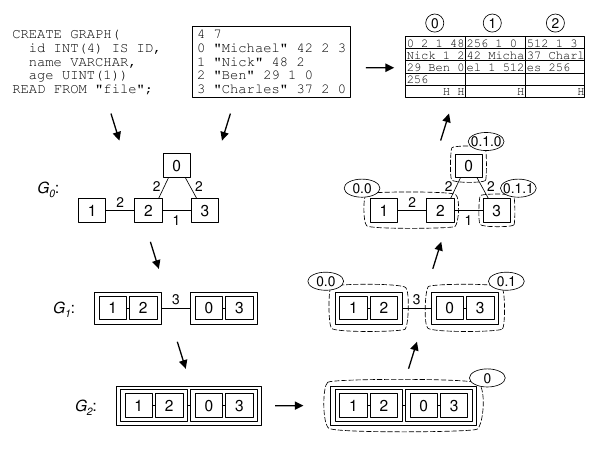
\includegraphics[keepaspectratio,width=0.7\textwidth]{img/06-rel_w/g-store.png}
        \end{center}
        \caption{A broad overview of the multilevel partitioning method applied by G-Store~\autocite{steinhaus2010g}.} 
        \label{g-store}
    \end{figure}

    
    In the next part of this section we are going to use the notions of a finer and a coarser graph a lot. Let therefore $G = G_0 = (V_0, E_0)$ the original graph, and $G_i = (V_i, E_i)$ the graph that was coarsened $i$ times.
    
    \subsection*{Coarsening}
    The coarsening phase of G-Stores partitioning algorithm is what is called heavy edge matching (HEM) in Karypis formulation of the algorithm as already mentioned. 
    Thus the algorithm takes $G_i$ as parameter and returns $G_{i+1}$ along with a projection $Z_{i+1}$ specifying which finer nodes maps to which coarser node.
    Coarsening proceeds in the original algorithm until a certain lower limit of vertices is reached.
    In the METIS implementation this is hard-coded to  $\max \left( 20k, 40 \log_2 k\right)$ where $k$ is a user defined parameter specifying the number of partitions.
    The algorithm used in G-Store keeps coarsening until there are no edges, i.e. only one vertex.
    It can thus be seen as a form of hierarchical agglomerative clustering~\autocite{hac} with the inverse edge weight acting as a distance function.
    
    Another modification is that in contrast to METIS~\autocite{karypis}, not only two edges are matched at a time but possibly many and that there is an upper limit to the vertex weights. 
    This depends on the coarsening factor $c(i) = \frac{|V_i| - |V_{i+1}|}{|V_i| - |\{v \in V | N_v = \emptyset \}|}$, with $i$ the level of coarsening, where $i=0$ it the original graph.
    The counter is the number of vertices that were reduced and the denominator is the number of nodes in the larger graph minus the irreducible nodes.
    Initially the allowed vertex weight $\theta$ is the size of a block.
    If this factor $c(i) < 0.3$ then the node weight $\theta$ is doubled as long as $\theta \leq 32$.
    Otherwise the number of nodes that are allowed to be matched is incremented.
        
    \subsection*{Turn-Around}
    In G-Store the turn-around simply assigns every vertex in the coarsest graph, whose weight is larger than the size of a block, a distinct partition number.
    The other nodes are added up until their weight reaches the size of a block and are assigned a partition number together.
    Thus the algorithm accepts a fully coarsened graph $G_i$ and returns the partition numbers for this graph $\phi_i$.
    
    This step is completely different than in the reference multilevel partitioning algorithm.

    
    \subsection*{Uncoarsening}
    The uncoarsening phase consists of three different steps that are performed per level:
    Projection, reordering and refinement.
    Projection constructs a first mapping, reordering swaps partitions and refinement exchanges nodes between partitions.
    Each iteration of the full uncoarsening procedure takes the coarser graph $G_{i+1}$ as an argument along with its the partition numbers $\phi_{i+1}$ and the mapping $Z_{i}$ and returns the one level uncoarsened graph $G_i$, along with the respective partition numbers $\phi_i$.
    The algorithm also defines a weight threshold per level. With $\overline{c}$ the average coarsening factor
    \[ \chi_i = \lfloor \frac{\text{block size}}{(1-\overline{c})^i} \rfloor. \]
    
    Further it defines three objective functions:\\
    The first function is closesly related to the minimal linear arrangement problem~\autocite{lewis1983computers} and expresses that nodes that share an edge shall be minimally far appart from each other.
    \[ \min C_1 = \min \sum_{(u,v) \in E} |\phi(u) - \phi(v)| \]
    The second objective function aims to reduce the overall number of edges between the partitions.
    \[\min C_2 = \min \sum_{(u,v) \in E)} \begin{cases}
        1 & \phi(u) \neq \phi(v) \\
        0 & \text{ otherwise}
    \end{cases}
\]
    The last objective function penalizes the number of blocks that are linked. That is in order to reduce the number of overall linked blocks according to~\autocite{steinhaus2010g}.
    \[ \min C_3 = \min \sum_{i \leq j} 
    \begin{cases}
        1 & \phi(u) = i \wedge \phi(v) = j, \ (u,v) \in E \\
        0 & \text{ otherwise}
    \end{cases}
    \]
    
    Finally there are two functions that are similar to the first objective function that are used in the projection step called tension and modified tension:
    The tension is the weighted distance between the block of the vertices that share and edge. Let $v \in V_i$.
    \[ t(v) = \sum_{u \in N_v} w_{(u,v)} \phi_i(v) - \phi_i(u)\]
     The modified tension is just the same, but instead of using the actual graph, one uses the coarser graph $G_{i+1}$ and the projection $Z_{i}$ to estimate the tension:
     \[ t'(v) = \sum_{u \in N_v} w_{(u, v)} \phi_{i+1}(Z(v)) - \phi_{i+1}(Z(u)) \]
    
        \subsubsection*{Projection}
        This part of the algorithm constructs a first version of the finer-grained partition numbers $\phi_i$ from the coarser ones $\phi_{i + 1}$.
        The enumeration follows a dewey numbering scheme.
        That is per level one place in the partition label is added. 
        If the vertex $\phi_{i+1}(Z(v)) = 2$ and vertex $\phi_i(v) = 1$, then the overall partition label of the vertex is $2\text{.}1$. 
        
        Per partition in the coarser level graph, the algorithm either simply assigns the same partition number to all nodes $v_i \in Z(\phi{i+1,j})$ in the finer graph $G_i$ that were clustered into the recpective coarser nodes, if the overall weight of the partition in the coarser graph is smaller than the weight threshold: $w_{\phi{i+1, j}} \leq \chi_i$.
        Otherwise the modified tension is computed is computed for all nodes of the partition in the finer graph $\forall v_i \in Z(\phi{i+1,j}): t'(v_i)$.
        The minimal tension is extracted, placed to the leftmost free position in the partition and the tensions of the neighbours are updated. 
        This is done repeatedly until all nodes are placed.
        During this step, each partition is marked with a flag, that is true, when it was created from nodes in the right half of the coarser partition.
        
        The projection differs vastly from the reference algorithm that just assigns the coarser partition number to all nodes in the finer grained graph.
                
        \subsubsection*{Reordering}
        This step is non-existent in the multilevel partitioning algorithm.
        When swapping the above created partitions, only $C_1$ changes, but not $C_2$ or $C_3$. Using the just created flags, groups are identified which span two half coarser partitions $\phi_{i+1,j}, \phi_{i+1,j+1}$. Per group the finer partitions are swapped as long as the overall absolute tension ($C_1$) decreases by some swap.
        In effect, this is a fix-point computation.
        
        \subsubsection*{Refinement}
        Finally the refinement step tries to optimize a weighted sum of all the objective functions by moving vertices to other partitions.
        In the reference algorithm this step simply uses the gain as defined in~\ref{kla}.
        Three used-defined parameters $\alpha, \beta, \gamma$ control the weighting, another one specifies the number of iterations that shall be executed $r$.
        In each iteration, the algorithm steps over the partitions $\phi_{i,j}$ and creates a two dimensional array $A$ of dimension $|\phi_{i,j}| \times |P_{i,j}|$ with $P_{i,j} = \{ \phi_i(u) | v \in \phi_{i,j}, u \in N_n\} \setminus \phi_{i,j}$.
        Each entry is defined with $v$ the vertex that is to be moved to partition $k$:
        \[ a_{v,k} = \alpha C_1 + \beta C_2 + \gamma C_3 + \lambda \]
        Where $\lambda$ penalizes overfull blocks or rewards the filling of less filled blocks.


    
\section{ICBL: Diffusion Set-based Clustering}
    Ya\c{c}ar and Gedik propose another method to form and order blocks~\autocite{yacsar2015scalable, yacsar2017distributed}. 
        
    They define one metric for each of the task:
    \textit{Block locality} is defined by the means of conductance and cohesiveness. 
    Conductance is defined as the ratio of edge cuts to total edges in a block:
    \[ C_d (B) = \frac{|\{ (u,v) \in E: |\{u,v\} \cap V_B| = 1\}|}{|\{ (u,v) \in E: |\{u,v\} \cap V_B| > 0\}|} \]
    Cohesiveness is the number of nodes in the same blocks that are connected by an edge divided by the number of theoretically possible edges, i.e. $|V|^2$ in a directed graph. The authors assume an undirected self-loop free graph, thus the number of possible edges is $\frac{|V| (|V| - 1)}{2}$.
    \[ C_h (B) = \frac{|\{ (u,v) \in E: u,v \in V_B \}|}{|V|^2} \]
    As conductance takes edges between blocks into account and cohesiveness meausures the edges within a block, they are complementary~\autocite{yacsar2015scalable}.
    Thus the locality of a block us defined as the geometric mean of the measures above, where the conductance is subtracted from one:
    \[ L(B) = \sqrt{C_h (B) \cdot (1 - C_d (B))} \]
    \textit{Ranking locality} is related to what we called tension before. 
    Here we do not measure it between partitions of the node but directly to the position in the order. 
    Let $v \in V$ a node and $r(v)$ a function that assigns a natural number in the range of $\{0, \dots, |V|-1\}$ to each vertex.
    \[ R (v) = \sum_{u \in N_v} r(v) - r(u) \]
    The locality of a block is then defined by one minus the normalized average distance for all vertices in the block:
    \[ R(B) = 1 - \frac{1}{(|V| - 1)} \sum_{v \in V_B} \frac{R(v)}{|N_v|} \]
    
    \begin{figure}[htp]
        \begin{center}
            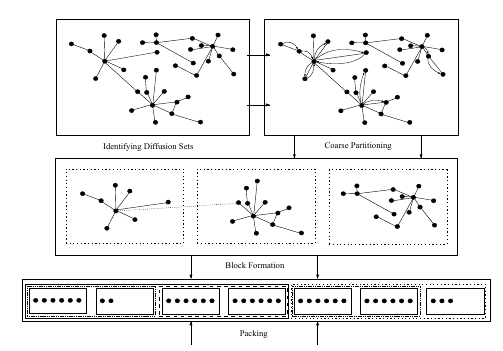
\includegraphics[keepaspectratio,width=0.8\textwidth]{img/06-rel_w/icbl.png}
        \end{center}
        \caption{A broad overview of the ICBL method by Ya\c{c}ar and Gedik~\autocite{yacsar2015scalable}.} 
        \label{icbl}
    \end{figure}

    ICBL is an acronym for the single steps performed by this algorithm. 
    It is designed to be implemented and executed using the map-reduce model.
    First ICBL extracts so called diffusion sets as features.
    Then it clusters the vertices based upon these features, to split the graph into subgraphs.
    After that it hierarchically clusters the subgraphs obtained in the previous step in order to form blocks.
    Finally the just formed blocks are ranked and layed out on disk.
    A brief visualization of the method is shown in~\ref{icbl}.
    
    \subsection*{Identify Diffusion Sets}
    The diffusion set $\mathcal{D}_v$ of a vertex $v \in V$ is a characterization of the surrounding of a vertex. 
    A surrounding means other vertices that are reachable in a certain number of steps.
    To identify the diffusion set, ICBL carries out $t$ random walks (\ref{rand-w}, \ref{random_walk}) of length $l$.
    The authors characterize a random walk using the vertices so from out definition we need to extract the multiset of vertices from the walk.
    
    For choosing the parameters $t$ and $l$ Ya\c{c}ar and Gedik propose heuristics: 
    For $t$, construct the cumulative degree distribution $f(d) \mapsto P(x \leq d)$ and chose the minimal degree value such that the derivative of the cumulative degree distribution $f'(d) = 1$. The value of the derivative was derived empirically.
    Regarding $l$ the authors make the assumotion that the network exihibits the small world phenomenon~\autocite{kleinberg2000small}.
    In a network that has that property, the probability is high that there exists a path between any two nodes $u,v \in V$ of length $\ln{|V|}$.
    In order to construct diffusion sets that are characterizing, the length of the random walk should not be too long as all nodes might be visitable then. Thus the heuristic for choosing $l$ is $1 + \lceil \frac{\ln |V|}{k} \rceil$ where $k$ is the number of clusters in the next step.
    
    \subsection*{Coarse Clustering}
    After generating the diffusion sets, the graph is clustered using a variation of the k-Means algorithm~\autocite{lloyd1982least}. 
    It is used to partition the graph into $k$ smaller subgraphs, such that the computationally more expensive agglomerative hierarchical clustering~\autocite{hac} algorithm that is used in block formation can be executed in parallel.
    Instead of using a geometric distance function (like the manhatten or the euclidean distance between points on a plane), an alternated version of the Jaccard distance function~\autocite{jaccard1912distribution} is used. 
    The Jaccard function $J(u, v) = 1 - \frac{\mathcal{D}_u \cap \mathcal{D}_v}{\mathcal{D}_u \cup \mathcal{D}_v}$, i.e. the distance is the number of common elements divided by the set of all elements in both sets. 
    The altered distance is adjusted for multisets:  
    \[J_w (u, v) = 1 - \frac{\sum_{x \in \mathcal{D}_v \cap \mathcal{D}_u} \min (w_{\mathcal{D}_v}, w_{\mathcal{D}_u})}{\sum_{x \in \mathcal{D}_v \cup \mathcal{D}_u} \max (w_{\mathcal{D}_v}, w_{\mathcal{D}_u})} \]
    First $k$ initial centers are chosen based upon the node degree and the distance to the already chosen centers.
    Then all nodes get assigned to the closest center. 
    After that the centers are updated, by building the union of all diffusion sets and use the vertex with the highest weight as new center.
    This is done until the centers do not change further.
    In order to determine the number of clusters, the authors propose a heuristic that is based on the available memory $M$ and the size of a vertex and the average diffusion set $s = \text{sizeof}(v) + \overline{\text{sizeof}(\mathcal{D})}$: 
    \[ k = \lceil \frac{s \cdot |V|}{\sqrt{0.8 \cdot M}} \rceil \]
    
    \subsection*{Block Formation}
    For each subgraph, agglomerative hierarchical clustering~\autocite{hac} is used to form blocks and label them for the ranking process.
    Each vertex starts in an own partition. 
    In every step the two closest partitions are merged. 
    The distance function here is the minimum of the previously defined weighted Jaccard distance of all nodes in the partition:
    \[ J_P (P_i, P_j) = \argmin_{u \in P_i, v \in P_j} J_w (\mathcal{D}_u, \mathcal{D}_v) \]
    Each partition maintains a label, that is used subsequently.
    In the beginning the node id is used as label. 
    When a potential merge would cause the so formed partition to exceed the block size, without one of the child partitions being already marked as block, the partition is marked as a block.
    Additionally the label is adjusted by appending a dot and a counter.
    If only one of the child partitions formed a block, the label of that partition is used.
    Finally when both children have formed a block before, their label is merged and a double colon is inserted in the middle.
    The algorithm terminates when all partitions are assigned to a block.
    To keep track of the uncaptured nodes in a partition where one child formed a block before an additional field is neccessary.    
    
    
    \subsection*{Layout}
    Finally, the tree is traversed to extract the so formed blocks and these blocks are sorted according to the label. 
    Finally each of the subgraphs is treated as vertex and the distance between them is the inverse of the number of edges between the subgraphs. Those with the lowest distance get merged and the whole graph is layed out to disk.
    

\section{Bondhu}
    Bondhu~\autocite{hoque2012disk} is a data layout technique for online social network data. 
    The authors define the cost of a placement similar to the ranking locality above, with $r$ defined as before: \[ \text{cost} = \sum_{(u, v) \in E} |r(v) - r(u)| \]   
    Without citing G-Store, Hoque and Gupta propose to use the multilevel partitioning algorithm implemented in METIS~\autocite{karypis} to partition the graph. Additionally the authors propose to use the Louvain method~\autocite{blondel2008fast} to find communities, but they don't provide results on this method. The louvain method is described in more detail in the next section. \\
    
    \begin{figure}[htp]
        \begin{center}
            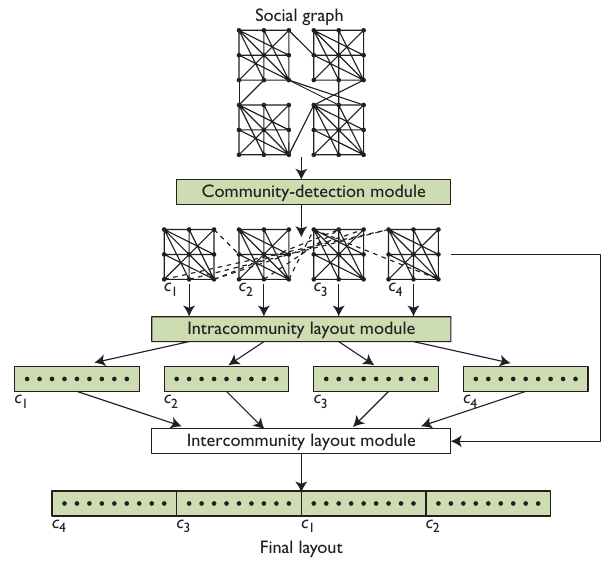
\includegraphics[keepaspectratio,width=0.8\textwidth]{img/06-rel_w/bondhu.png}
        \end{center}
        \caption{Broad steps performed by the bondhu algorithm~\autocite{hoque2012disk}.} 
        \label{bondhu-fig}
    \end{figure}

    The authors propose an incremental placement schema within a block:
    Place the node with the highest degree in the middle of the block, then select the node with the heaviest edge connected to the first node and place it next to the first node. 
    After these two placements, a new graph is created, where the two already placed nodes are merged and their relationships are aggregated. 
    The node with the next heaviest edge is selected and placed alternatingly. The previous two steps are repeated until all nodes are placed within blocks.
    This is done for every community.
    In the final part of the method, the intercommunity layout is derived. 
    Here each community is a vertex and the edges between those are just the accumulated edges of the underlying graph. 
    After creating the graph the previous alternating placement schema is applied.
